\section{Auswertung}
\label{sec:Auswertung}

\subsection{Bestimmung des Planckschen Wirkungsquantum aus dem Photostrom}
  Es wurden für verschiedene Spektrallinien die Anodenspannung variiert und der resultierende
  Strom zwischen Anode und Anode gemessen. Folgende Werte wurden ermittelt:
  \begin{table}[H]
    \centering
    \caption{Messwerte der roten Spektrallinie}
    \label{tab:fiesemoepp}
    \begin{tabular}{c c}
     \toprule
      U [V]& I[nA]\\
     \midrule
      2    & 0.025  \\
      1.75 & 0.02   \\
      1.5  & 0.018  \\
      1.25 & 0.016  \\
      1    & 0.0143 \\
      0.75 & 0.012  \\
      0.5  & 0.01   \\
      0.25 & 0.0075 \\
      0.02 & 0.002  \\
     -0.2  & 0.001  \\
     -0.4  & 0      \\
     -0.6  & 0      \\
     \bottomrule
    \end{tabular}
  \end{table}
  \begin{table}[H]
    \centering
    \caption{Messwerte der grünen Spektrallinie}
    \begin{tabular}{c c}
     \toprule
      U [V]& I[nA]\\
     \midrule
     2    & 1.4  \\
     1.75 & 1    \\
     1.5  & 0.95 \\
     1.25 & 0.8  \\
     1    & 0.7  \\
     0.75 & 0.6  \\
     0.5  & 0.5  \\
     0.25 & 0.4  \\
     0.02 & 0.3  \\
    -0.2  & 0.2  \\
    -0.4  & 0.09 \\
    -0.6  & 0.01 \\
    -0.8  & 0    \\
     -1    & 0    \\
     \bottomrule
    \end{tabular}
  \end{table}  
  \begin{table}[H]
    \centering
    \caption{Messwerte der blauen Spektrallinie}
    \begin{tabular}{c c}
     \toprule
      U [V]& I[nA]\\
      \midrule
      2    & 2.1  \\
      1.75 & 1.75 \\
      1.5  & 1.55 \\
      1.25 & 1.4  \\
      1    & 1.23 \\
      0.75 & 1.1  \\
      0.5  & 0.95 \\
      0.25 & 0.8  \\
      0    & 0.7  \\
     -0.2  & 0.5  \\
     -0.4  & 0.3  \\
     -0.6  & 0.2  \\
     -0.8  & 0.15 \\
     -1    & 0    \\
     \bottomrule
    \end{tabular}
  \end{table} 
  \begin{table}[H]
    \centering
    \caption{Messwerte der gelben Spektrallinie im Bereich von 2 V bis -1 V}
    \begin{tabular}{c c}
     \toprule
      U [V]& I[nA]\\
      \midrule
      2    & 0.6   \\
      1.75 & 0.55  \\
      1.5  & 0.5   \\
      1.25 & 0.45  \\
      1    & 0.4   \\
      0.75 & 0.35  \\
      0.5  & 0.28  \\
      0.25 & 0.22  \\
      0.02 & 0.15  \\
     -0.2  & 0.1   \\
     -0.4  & 0.018 \\
     -0.6  & 0     \\
     -0.8  & 0     \\
     -1    & 0     \\
     \bottomrule
    \end{tabular}
  \end{table} 
  \begin{table}[H]
    \centering
    \caption{Messwerte der gelben Spektrallinie im Bereich von 19 V bis -0.2 V}
    \label{tab:idle}
    \begin{tabular}{c c}
     \toprule
      U [V]& I[nA]\\
      \midrule
       19     & 1.43  \\
       18     & 1.4   \\
       17     & 1.37  \\
       16     & 1.3   \\
       15     & 1.27  \\
       14     & 1.26  \\
       13     & 1.25  \\
       12     & 1.2   \\
       11     & 1.19  \\
       10     & 1.17  \\
        9     & 1.1   \\
        8     & 1.07  \\
        7     & 1     \\
        6     & 0.9   \\
        5     & 0.92  \\
        4     & 0.84  \\
        3.5   & 0.78  \\
        3     & 0.72  \\
        2.5   & 0.63  \\
        2     & 0.45  \\
        1.75  & 0.4   \\
        1.5   & 0.32  \\
        1.25  & 0.25  \\
        1     & 0.2   \\
        0.75  & 0.175 \\
        0.5   & 0.12  \\
        0.25  & 0.05  \\
        0.002 & 0.012 \\
       -0.2   & 0     \\
     \bottomrule
    \end{tabular}
  \end{table} 
  \noindent Die für die verschiedenen Spektrallinien aufgenommenen Daten werden
  in Tabelle \ref{tab:fiesemoepp} bis Tabelle \ref{tab:idle} wiedergegeben.
  Für die Analyse anhand der Funktion $\sqrt{I}=aU+b$ sind in Abbildung \ref{fig:plot} 
  bis \ref{fig:scheisse} die Wurzel des Photostromes gegen die angelegte Spannung für jede betrachtete
  Spektrallinie
  aufgetragen. Diese werden grafisch auf Linearität untersucht. Für die als linear befundenen Teile 
  der jeweiligen Messwertfolge wurde mittels Python eine lineare Regression 
  mit der Funktion $\sqrt{I}=aU+b$ angefertigt. Zunächst sind nun die Abbildungen dargestellt, 
  danach folgen die Erläuterungen und Ergebnisse.
  Die Messwerte für die rote Spektrallinie mit einer Wellenlänge von $\lambda = 614 \si{\nano\meter}$
  ist in folgender Abbildung dargestellt.
  \begin{figure}[H]
    \centering
    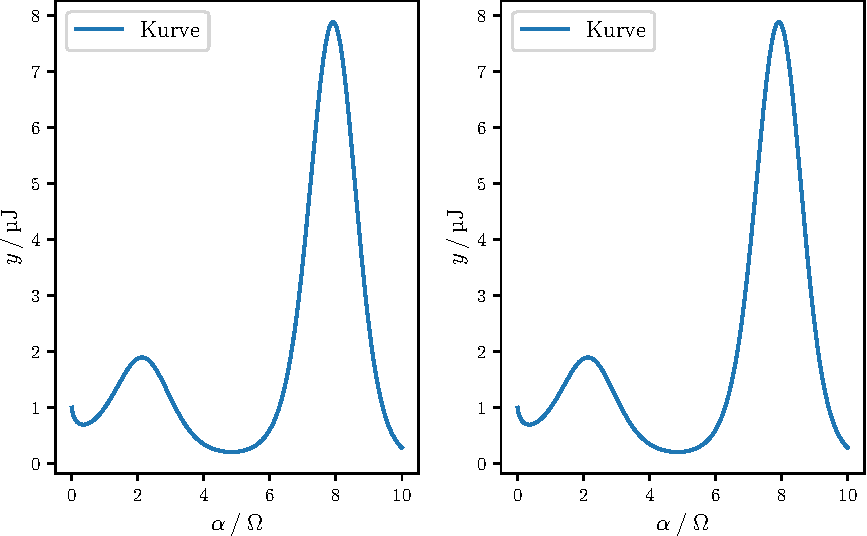
\includegraphics[scale=0.8]{build/plot.pdf}
    \caption{Messwerte und lineare Regression der roten Spektrallinie}
    \label{fig:plot}
  \end{figure}
  Die Messwerte für die güne Spektrallinie mit einer Wellenlänge von $\lambda = 546 \si{\nano\meter}$
  ist in folgender Abbildung dargestellt.
  \begin{figure}[H]
    \centering
    \includegraphics[scale=0.8]{build/fuckyou.pdf}
    \caption{Messwerte und lineare Regression der grünen Spektrallinie}
    \label{fig:fuck}
  \end{figure}
  Die Messwerte für die blaue Spektrallinie mit einer Wellenlänge von $\lambda = 492 \si{\nano\meter}$
  ist in folgender Abbildung dargestellt.
  \begin{figure}[H]
    \centering
    \includegraphics[scale=0.8]{build/hurensohn.pdf}
    \caption{Messwerte und lineare Regression der blauen Spektrallinie}
    \label{fig:hure}
  \end{figure}
  
  Für die gelbe Spaktrallinie mit einer Wellenlänge von $\lambda = 577.579 \si{\nano\meter}$
  wurden zwei Messreihen durchgeführt. Die erste jener ist in folgender Abbildung dargestellt.
  \begin{figure}[H]
    \centering
    \includegraphics[scale=0.8]{build/fresse.pdf}
    \caption{Messwerte und lineare Regression der gelben Spektrallinie}
    \label{fig:fresse}
  \end{figure}
  In der folgenden Abbildung \ref{fig:scheisse} ist die zweite Messreihe für die gelbe Spektrallinie
  dargestellt.
  \begin{figure}[H]
    \centering
    \includegraphics[scale=0.8]{build/verdammtescheiße.pdf}
    \caption{Messwerte und lineare Regression der gelben Spektrallinie}
    \label{fig:scheisse}
  \end{figure}
  
  In Tabelle \ref{tab:hirntoter} sind jeweils der Begin und das Ende der linearen Teile der Messdaten
  für die jeweilige Spektrallinie dargestellt. Es wird für jede Spektrallinie von $U_a$ bis $U_b$ 
  die lineare Regression durchgeführt.
  \begin{table}[H]
    \centering
    \caption{Parameter der linearen Regressionen}
    \label{tab:hirntoter}
    \begin{tabular}{c c c}
     \toprule
      $\lambda$ [nm] & $U_{a}$ [V] & $U_{b}$ [V] \\
      \midrule
      614     & -0.2 & 0.5  \\
      577.579 & -0.2 & 2.5  \\
      577.579 & -0.6 & 0.02 \\
      546     & -0.8 & 0.02 \\
      434     & -1   & 0    \\
     \bottomrule
    \end{tabular}
  \end{table} 
  Die durch die lineare Regression bestimmten Koeffizienten und den Grenzspannungen $U_G$,
  der sich aus den Schnittpunkten mit der Spannungsachse ergibt, sind in Tabelle 
  \ref{tab:affenarsch} dargestellt. 
  
  \begin{table}[H]
    \centering
    \caption{Parameter der linearen Regressionen}
    \label{tab:affenarsch}
    \begin{tabular}{c c c c}
     \toprule
      $\lambda$ [nm] & a & b & $U_G$ [nV]\\
      \midrule
      614     & 0.106 ± 0.018&0.051 ± 0.005&-0.47867  \\
      577.579 & 0.257 ± 0.015&0.175 ± 0.021&-0.683269 \\
      577.579 & 0.598 ± 0.169&0.395 ± 0.044&-0.660231 \\
      546     & 0.721 ± 0.087&0.561 ± 0.033&-0.77884  \\
      434     & 0.579 ± 0.054&0.817 ± 0.026&-1.41017  \\
     \bottomrule
    \end{tabular}
  \end{table} 
  \noindent Durch Umpolen werden die Werte für $U_G$ positiv. Um nun die Austrittsarbeit aus der Photokathode
  und das Plancksche Wirkungsquantum zu bestimmen, wird mit den erhaltenen Gegenspannungen 
  mit zugehörigen Lichtfrequenzen erneut eine lineare Regression durchgeführt. Die bestimmten
  Gegenspannungen $U_G$ sind in der folgenden Grafik \ref{fig:torte} gegen die zugehörigen 
  Wellenlängen aufgetragen.
  \begin{figure}
    \centering
    \includegraphics{torte.pdf}
    \caption{}
    \label{fig:torte}
  \end{figure}
  Mit einer linearen Regression in Python der Ausgleichsgeraden $U_G=a\cdot f +b$ 
  werden die Koeffizienten
  \begin{align*}
    a = (4.46 ± 0.18) \cdot 10^{-15}\\
    b = 1.66 ± 0.1
  \end{align*}
  bestimmt. Aus Gleichung \ref{eqn:bilanz} folgt, dass die Steigung a dem Bruch $\dfrac{h}{e}$ und 
  der Achsenabschnitt b der Austrittsarbeit in eV entspricht. Somit ergibt sich
  \begin{align*}
    h = 4.46 \cdot 10^{-15} eVs\\
    W_A = 1.66 eV.
  \end{align*}
  nachdem die Umrechnung von Nanometern in Metern erfolgt ist.

\subsection{Betrachtung des Photostroms in Abhängigkeit von der Spannung}
  Nun wird bei einer Wellenlänge von $\lambda = 578$ nm der Photostrom bei einer Variation
  der angelegten Brems- bzw. Beschleunigungsspannung von -0.2 V bis 19 V gemessen. Die
  Daten sind in Tabelle \ref{tab:idle} gelistet und in Abbildung \ref{fig:scheisse} dargestellt.
  Es ist ersichtlich, dass es einen Sättigungswert gibt, gegen den die Kurve strebt.
  Dieser kommt durch die konstante Intensität des bestrahlenden Lichtes
  zustande. Die Anzahl der austretenden Elektronen ist nämlich proportional zu der
  Intenssität des einfallenden Lichtes.
  Ab einem gewissen Punkt werden nicht mehr Elektronen vom Licht freigesetzt
  als von der Anode angezogen. 
  Da die Elektronen beim Austritt über verschiedene kinetische Energien verfügen, 
  und einen Impuls in Unterschiedliche Richtungen aufweisen, und daher teilweise die Anode 
  verfehlen, wird der Sättigungswert asymptotisch erreicht. Der Sättigungswert hängt also 
  von der Oberfläche der Anode sowie der Intensität ab.\\
  Auch bei der Spannung $U_G$ gibt es keinen Knick, sondern eine asymptotische Annäherung.
  Diese exestiert aus dem selben Grund. Auch wenn keine Spannung anliegt, gibt es Elektronen,
  die kinetischische Energie in Richtung der Anode besitzen, sodass trotzdem ein Strom zwischen 
  Kathode und Anode entsteht. \\
  Weiterhin wurde im Bereich der Gegenspannung, also bei $U_G \leq U$ ein entgegengesetzer 
  Stromfluss gemessen. Dieser ist durch die Beschichtung der Kathode zu erklären. Diese
  ist so gewählt, dass diese eine geringe Austrittsarbeit für Elektronen besitzt. Sie 
  verdampft bereits bei geringen Temperaturen, sodass sich ionisierte Atome von der Kathode 
  lösen und aufgrund Ihrer positiven Ladung zur Anode fliegen.\\

%Miks seda ei tööta?